\documentclass[letterpaper,11pt]{article}

\usepackage{classDM}
\usepackage{hyperref}
\usepackage[normalem]{ulem}
\usepackage{inconsolata}
\usepackage{enumitem}
\usepackage{caption}

\usepackage{float} % For the H placement specifier
\usepackage{subcaption}

\usepackage[
backend=biber,
style=numeric,
]{biblatex} %Imports biblatex package
\addbibresource{sources.bib} %Import the bibliography file

\usepackage{bessex}

\title{Media Representation as a\\ 
\vspace{.1in} 
Predictor for Climate Policy Outcomes}
\author{Ben Essex, Emma Kerr}
\date{} 

\begin{document}
\maketitle

%\end{titlepage}

%%%%%%%%%%%%%%%%%%%%%%%%%%%%%%%%%%%%%%%%%%%%%%%%%%%%
%%%%%%%%%%%%%%%%%%%%%%%%%%%%%%%%%%%%%%%%%%%%%%%%%%%%
%%%%%%%%%%%%%%%%%%%%%%%%%%%%%%%%%%%%%%%%%%%%%%%%%%%%
\section{Introduction}

\vspace{.1in}

% Problem and motivation
\quad\textbf{Problem, Motivation, and Key Idea.}
Climate change is being increasingly viewed as an existential crisis. Legislators in the United States have, in recent years, stepped up efforts to enact policies that might address this crisis. In a representative democracy, legislators are generally expected to act in accordance with the public good and in line with the views of their constituencies. This results in a complex interplay of news media, public opinion, and special interests, resulting in the enactment or failure of these policies. To many, the success of climate policy--its ``outcome"--is viewed as a question so important that its answer may dictate the very future of human life itself. As a result, there is great interest and value in better empirically understanding the complex dynamic by which these outcomes are produced.

This project seeks to address this question and to analyze the nature of the dynamic between how media represents climate policies and the political outcomes for those policies. We examine factors such as amount of media coverage, media source bias, sentiment on climate policy, and policy outcomes. A successful result for this study would be to make a contribution to the field of policy analysis, in the form of new techniques or analytic results. In this study, we introduce advanced methods in data acquisition, ETL, feature engineering, and analysis that are novel to this field.\\

\textbf{Previous Works.}
Studies to date on this topic have produced interesting results with a less quantitative approach. For example, one article focuses on normative questions \cite{boykoff2007climate}. Another examines the connection between viewership of popular cable news channels and viewer beliefs on climate change \cite{feldman2012climate}. However, previous works have generally examined this topic neither at massive scale nor with advanced data mining techniques.

%%%%%%%%%%%%%%%%%%%%%%%%%%%%%%%%%%%%%%%%%%%%%%%%%%%%
%%%%%%%%%%%%%%%%%%%%%%%%%%%%%%%%%%%%%%%%%%%%%%%%%%%%
%%%%%%%%%%%%%%%%%%%%%%%%%%%%%%%%%%%%%%%%%%%%%%%%%%%%
%%%%%%%%%%%%%%%%%%%%%%%%%%%%%%%%%%%%%%%%%%%%%%%%%%%%

\section{Data}

\vspace{.1in}

\subsection{Data Collection, Processing, and Feature Engineering}
Raw data was collected from several sources, and most underwent significant processing and transformation to be useful for analysis.\\

\quad\textbf{News Articles.} The corpus of news articles in this study was entirely sourced using the AYLIEN News API \cite{aylien}. In order to consume this API, we acquired an trial API key and built a harness around the API client. Once we developed a list of terms pertaining to policies under study (see \hyperref[dcap:ClimatePol]{Climate Policy}), we queried AYLIEN for any articles containing these terms, building a \verb|documents.json| file with over 40,000 articles since the beginning of the query window (27 months prior--the earliest AYLIEN would allow us to query). We stored each document with the document id, the published date, the article body, and the publishing source. Most of the time spent in this collection phase involved developing the harness and tweaking parameters to avoid exhausting AYLIEN's rate limit. The actual time to collect was less than a few hours using the harness.\\

\textbf{Climate Policy.}\label{dcap:ClimatePol} In order to produce a list of climate policies (bills and resolutions) to assess, we began with a manually generated list of terms related to climate (e.g. ``Climate Change," ``Carbon Dioxide," ``Methane," etc). We acquired an API key to the free ProPublica Congress API, for which we built another harness. Using this harness and the list of key terms, we queried the ProPublica API for bill topics or ``subjects" relevant to our key terms list \cite{propublica_congress_api}. When we had a list of subjects, we queried the ProPublica API for bills listed under those subjects. These bills comprise our list of ``climate policies." Like the news articles, the list of bills was restructured to fit a purpose-built JSON schema to ease storage and analysis. In addition to identifiers for each bill (including title, bill number, introduced date, etc.), we separately queried ProPublica for information on the latest House and/or Senate vote for each bill. For each vote, we computed and saved the overall proportion of votes for adoption of the bill, as well as the proportion for each party.

Due to the nature of the American legislative system, relatively few bills ever see a floor vote (e.g., only around 20 of the 138 bills we focused on). This meant clever feature engineering would be required to operationalize the outcome or ``success" of a bill. Since success could perhaps be measured in terms of the bill's distance from becoming public law, an ordinal representation for the bill's latest major action could be used as a measure of its success. For example, a bill that becomes public law might be assigned a \verb|last_action_ordinal| of 17, whereas a bill that has only just been introduced would be at 0. In order to determine the value of this new feature for each bill, we developed a harness to consume the U.S. Library of Congress API \cite{loc_api}. Using the bill data already acquired, we queried the API for the last major action code and last major action date. Since last major action code increments as bills progress through the legislative process (see \hyperref[appendix:B]{Appendix B}), we identified an opportunity to convert this value into an ordinal representation, which was saved along with the unix timestamp of the action in the bill data JSON file.\\

\textbf{Media Bias.} Another key factor in capturing the interplay of public opinion and policy outcome is certainly source bias. When dealing with policy, news sources are likely to present information in a way that aligns with the bias of the source. Furthermore, there is a human tendency to primarily consume sources with agreeable views, and this means the group primarily exposed to a biased representation often holds the same bias as the media outlet presenting it. The implications for public opinion and consequently policy outcomes are clear. So, in order to collect bias data for each news source, we utilized AllSides.com's source bias ratings, as manually annotated by their editors \cite{allsides_bias_ratings}. We then developed a tool to systematically access the source associated with every article acquired from AYLIEN and scrape AllSides.com for the bias rating of the source, saving an ordinal categorical bias rating $[1.0,\ 2.0,\ 3.0,\ 4.0,\ 5.0]$ with every document for which the source had an associated bias rating.\\

\textbf{Media Sentiment.} The last key piece of raw data needed is media sentiment. Core to an article's representation of a policy is the sentiment with which it presents it. Performing sentiment analysis at scale and in relation to climate policy would be a key enabling factor for a great deal of analysis of the dynamic between media representation and policy outcomes. Engineering a feature to capture sentiment was a multi-step process. We began with the bill terms list used for querying AYLIEN. This included bill number in multiple forms (e.g., H.R.1, H.Res. 1, etc.) and bill title. We tokenized each term using the spaCy English language tokenizer and created a mapping of start tokens to the corresponding token group. Then, we tokenized each article and iterated through each tokenization. If a token matched one of our starting tokens, the subsequent tokens were checked against the saved token group. If a match was found, a ``window" was saved--containing the matching text, the document id, the start and end indices in the document for the match, and an assigned instance id. By saving the start and end indices, later analysis could make use of a variable $\frac{k}{2}$ tokens on either side of the match.

After producing over 4,700 instances, we randomly sampled 56 instances to manually annotate. For each instance, we examined the $k$-gram in the text that subsumed the matching tokens ($k$ not including the number of tokens in the match itself). For this study, we set $k$ to 50 as a starting point that might produce sufficient context to accurately annotate instances. We labeled each instance as \verb|positive|, \verb|neutral|, or \verb|negative| about the climate policy in question. These instances became our training examples for $3 \times 19$ shot learning and subsequent sentiment classification using FLAN-T5 XL \cite{flan-t5-xl}. Since FLAN-T5 was limited to 512 tokens in the input, out of necessity we developed an extension of few-shot learning in which we chose, without replacement, 3 training examples to present prior to the instance to be classified. For each of our 4,700+ instances, we would shuffle our training instances, then divide these instances into non-overlapping groups of 3 each. For each training set, we used FLAN-T5 with 3 beams in a beam search and saved the top 3 return sequences with scores. We computed normalized probabilities for each sentiment based on the probability distribution produced by running the softmax function over the last logit of each return sequence. We then saved the average probability for each sentiment polarity across each of the training sets, for all 4,700 instances. The final classification phase took less than 2 hours.

%%%%%%%%%%%%%%%%%%%%%%%%%%%%%%%%%%%%%%%%%%%%%%%%%%%%
%%%%%%%%%%%%%%%%%%%%%%%%%%%%%%%%%%%%%%%%%%%%%%%%%%%%
%%%%%%%%%%%%%%%%%%%%%%%%%%%%%%%%%%%%%%%%%%%%%%%%%%%%
%%%%%%%%%%%%%%%%%%%%%%%%%%%%%%%%%%%%%%%%%%%%%%%%%%%%

\section{Analysis}
% TODO: this would be a great place to put a regression of party predicting likelihood to vote for climate legislation!!

\begin{figure}[htbp]
    \centering
    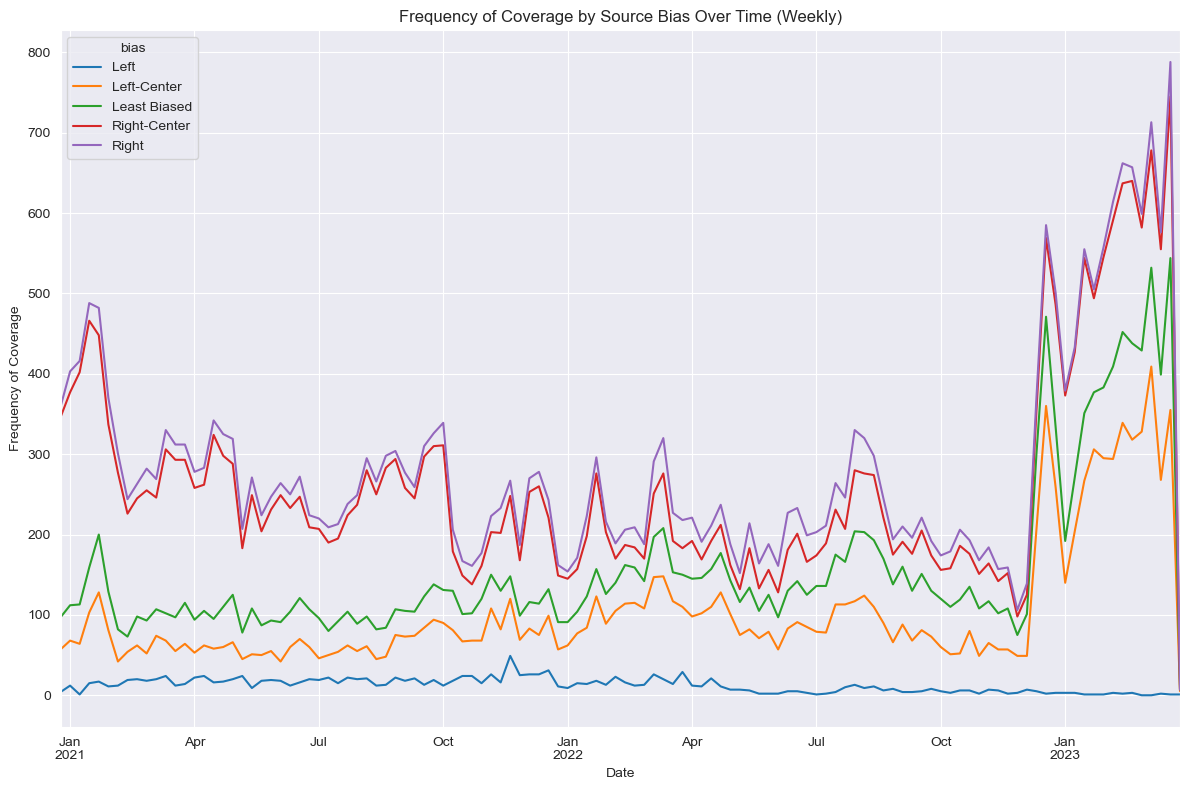
\includegraphics[width=\textwidth]{figs/fig_5.png}
    \caption{Sum of weekly climate policy coverage by source bias}
    \label{fig:fig1}
\end{figure}

\subsection{Bias and Coverage}
It is an oft-quoted assertion in the public affairs world that ``any coverage is good coverage." Irrespective of whether this hypothesis is borne out by the data, we can accept that greater volume of coverage is likely to translate to greater public awareness of climate policy. At any rate, we can see that it would be valuable to examine the frequency of coverage provided by sources of varying bias. In \hyperref[fig:fig1]{Figure 1}, we see volume of coverage, by source bias, over time (sampled weekly). The greatest volume of coverage seems to come from sources with a right-center bias, but interestingly, this fluctuates. Certain time periods have significantly more coverage from right-leaning sources, while other periods see the reverse.

For example, peak coverage volume was in late November 2021 for left sources, March 2023 for left-center and center, mid-January 2021 for right-center, and end of July 2022 for right. Additional analysis could be useful here to better understand the corresponding legislative events for these coverage peaks.

\begin{figure}[htbp]
    \centering
    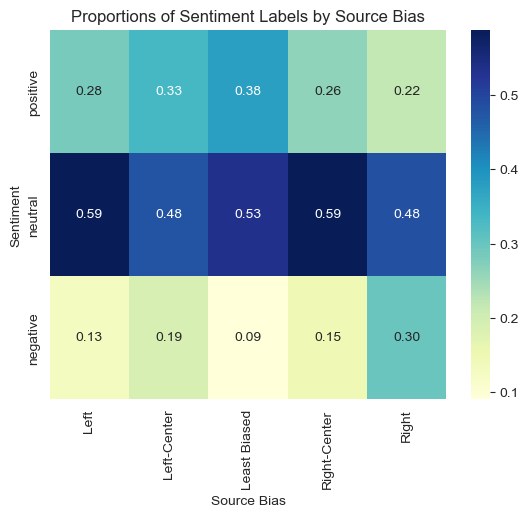
\includegraphics[width=0.55\textwidth]{figs/fig_3.png}
    \caption{Heat map of source bias and sentiment}
    \label{fig:heatmap}
\end{figure}

\subsection{Bias and Sentiment}
A common understanding of modern American politics is that groups with bias toward the left tend to embrace climate policy, while groups near the right tend to reject the notion that climate policy is necessary, for one reason or another. Certainly we have seen this to be the case for the Republican party in our dataset, as the proportion of Republicans voting to adopt climate policies tends always lower than the proportion of Democrats. One question, then, is whether this is connection is reflected in media bias vs sentiment toward climate policy. By cross-tabulating source bias with sentiment, we observe  a few trends in \hyperref[fig:heatmap]{Figure 2}. For example, we see that sources with right bias tend to be the most likely to present climate policy with negative sentiment. Center and left-center sources tend to be the most likely to present climate policy with positive sentiment, while all sources present climate policy with neutral sentiment in a plurality of cases.\\


\vspace{.1in}
\subsection{Regression of Article Sentiment vs Bill Success}
    \textbf{Sentiment vs Bill Ordinality}
    This analysis considers the 4,700 bill windows from the data collection step. These are the article windows collected from our AYLIEN scrape that could be re-matched to individual bill numbers. These matched windows, the sentiment assigned to them by FLAN-T5, and the bill's success all contribute for the data used in these regression models. 

    This study in particular only considers the subset of windows mentioning bills that were published before the last action of that specific bill. This is in hopes of capturing how the sentiment of media published before a bill affects the ``success" of the particular bill. Success was measured by both the assigned ordinality of the data collection step, and the proportion of the House/Senate voting in favor of a particular bill. 

    Each regression also assigns bill sentiment to be the highest confidence of all 3 categories and sets the other categories to be 0. This is in hopes of streamlining the data and reducing noise that may be introduced by having multiple sentiment categories assigned to the same bill. In addition, the proportion of positive, negative, and neutral sentiment assigned to each bill window is aggregated and averaged and used as an independent variable in the regression models. \\

    \begin{figure}[ht]
      \centering
      \begin{subfigure}{0.45\textwidth}
        \centering
        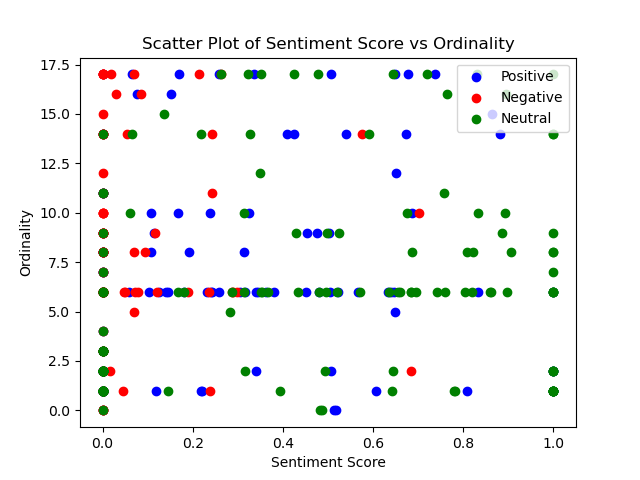
\includegraphics[width=\linewidth]{figs/foo2.png}
        \caption{}
        \label{fig:sub1}
      \end{subfigure}
      \hfill % Optional horizontal space
      \begin{subfigure}{0.45\textwidth}
        \centering
        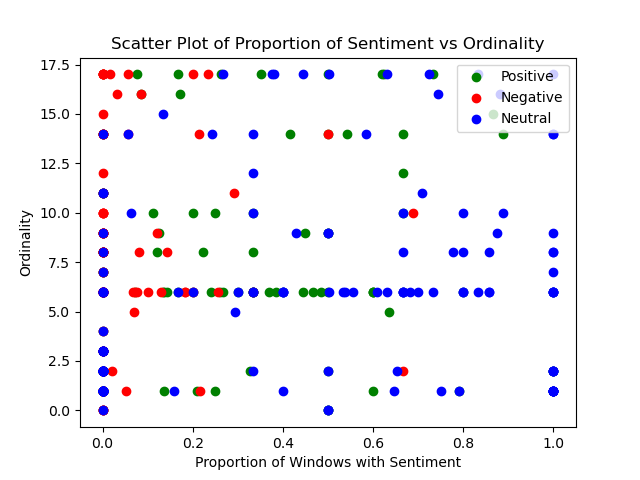
\includegraphics[width=\linewidth]{figs/foo.png}
        \caption{}
        \label{fig:sub2}
      \end{subfigure}
      \caption{}
      \label{fig:main}
    \end{figure}
    
    Linear regression of \href{fig:scatterplot}{Figure 3 a} gives a positive sentiment coefficient of 5.002, negative coefficient of 8.4371, and neutral of 3.7952 suggesting that as media increases in positive, negative, or neutral sentiment confidence, a bill is more likely to have more action taken towards passing. This, of course, is a weak conclusion as the $R^2$. is ~0.25 for positive and negative sentiment and ~0.19 for neutral sentiment, although the results found are interesting and warrant further investigation.
    
    \href{fig:scatterplot}{Figure 3 b} shows a similar plot on the proportion of positive, neutral, and negative instances per bill. A similar conclusion can be made with a negligible $R^2$ value. \\
    
    \textbf{Positive and Negative Sentiment vs Congress Vote Proportion.} 
    This next regression uses the climate policy bills that were voted on by Congress. This subset only included 20 bills, however, the findings are still significant and provide insight into the relationship between public opinion and climate policy. The previous filtering methods (choosing windows before last action date, including only the subset of windows mentioning the bill) are also included here. 

    This analysis explores the relationship between the proportion of majorly positive, neutral, and negative windows and proportion of Congress members voting in favor of the bill. 

    \begin{figure}[ht]
      \centering
      \begin{subfigure}{0.45\textwidth}
        \centering
        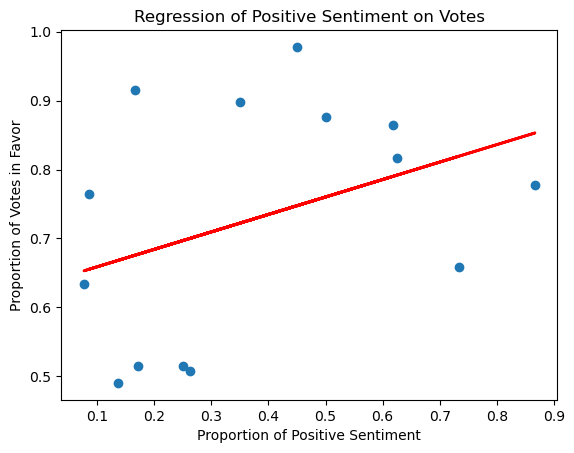
\includegraphics[width=\linewidth]{figs/fig_13.png}
        \caption{Correlation Coefficient: 0.2533479066825248 \\ $R^2$: 0.14178738044276173}
        \label{fig:sub21}
      \end{subfigure}
      \hfill % Optional horizontal space
      \begin{subfigure}{0.45\textwidth}
        \centering
        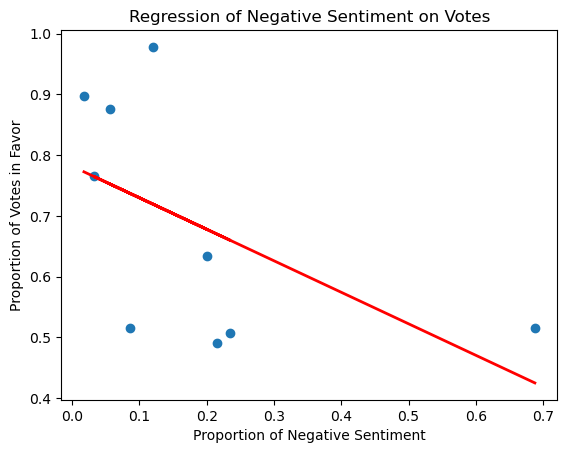
\includegraphics[width=\linewidth]{figs/fig_14.png}
        \caption{Correlation Coefficient: -0.55109343709179 \\ $R^2$: 0.3492484170148309}
        \label{fig:sub22}
      \end{subfigure}
      \caption{}
      \label{fig:main2}
    \end{figure}

The third plot for neutral sentiment has not been included as the $R^2$ value is negligible (0.002). However, these two plots provide some evidence that the more positive media sentiment is, the more likely a bill is to be passed, and the opposite is true for negative sentiment, with a stronger $R^2$ value. 

%%%%%%%%%%%%%%%%%%%%%%%%%%%%%%%%%%%%%%%%%%%%%%%%%%%%
%%%%%%%%%%%%%%%%%%%%%%%%%%%%%%%%%%%%%%%%%%%%%%%%%%%%
%%%%%%%%%%%%%%%%%%%%%%%%%%%%%%%%%%%%%%%%%%%%%%%%%%%%
%%%%%%%%%%%%%%%%%%%%%%%%%%%%%%%%%%%%%%%%%%%%%%%%%%%%


% \section{Ethics}

% \vspace{.1in}

% \begin{enumerate}
%     \item Ethical considerations and implications of the study. (For example, systematic bias not in the news articles but in the provider, AYLIEN; bias ingrained in FLAN-T5-xl)
% \end{enumerate}

%%%%%%%%%%%%%%%%%%%%%%%%%%%%%%%%%%%%%%%%%%%%%%%%%%%%
%%%%%%%%%%%%%%%%%%%%%%%%%%%%%%%%%%%%%%%%%%%%%%%%%%%%
%%%%%%%%%%%%%%%%%%%%%%%%%%%%%%%%%%%%%%%%%%%%%%%%%%%%
%%%%%%%%%%%%%%%%%%%%%%%%%%%%%%%%%%%%%%%%%%%%%%%%%%%%

\subsection{Sentiment and Bill Success over Time}
Though our regressions show sentiment explains relatively little variation in bill success, it is worth analyzing trends in sentiment and bill success over time. In \hyperref[fig:heatmap-time]{the heatmap} below, we can identify period of relatively negative sentiment and periods of relatively positive sentiment. For this heatmap, the volume of instances with predominantly negative sentiment was subtracted from the volume with predominantly positive. Higher sentiment score means more positive coverage in that period.

\begin{figure}[htbp]
    \centering
    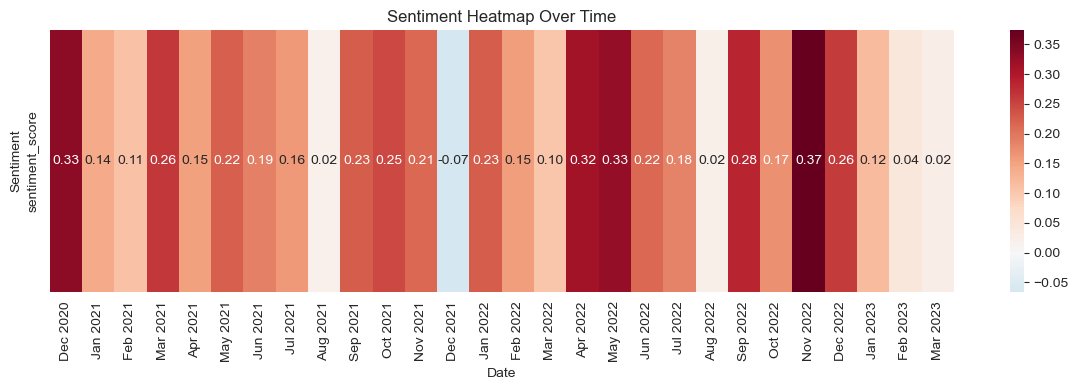
\includegraphics[width=0.85\textwidth]{figs/fig_8.png}
    \caption{Heat map sentiment over time}
    \label{fig:heatmap-time}
\end{figure}

Looking at the heatmap, we can see period of relative negativity--e.g., around Aug 2021, Dec 2021, and Aug 2022--as well as period of relative positivity--Dec 2020, May 2022, Nov 2022. In \hyperref[fig:prop-sent-time]{Figure 6}, we see some interesting dynamics in sentiment and bill success. In some cases--i.e., late 2021, April 2022, others--sentiment appears to drop rapidly before bill success drops. In other cases, bill success seems to preemptively move in tandem with positive sentiment. For example, the latter half of 2022 looks as though bill success to some extent predicts movements in sentiment. This makes sense logically, as articles discussing bills actions may be classified with the corresponding sentiment.

\begin{figure}[htbp]
    \centering
    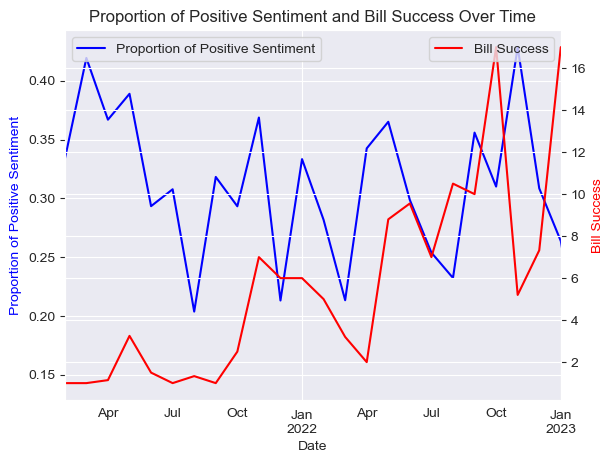
\includegraphics[width=0.55\textwidth]{figs/fig_9.png}
    \caption{Proportion of positive sentiment, bill success over time}
    \label{fig:prop-sent-time}
\end{figure}



\section{Drawbacks, Deficiencies, and Obstacles}

\vspace{.1in}

\quad This study met a number of unexpected obstacles; each of which resulted in deficiencies in the data or analysis to varying degrees. Chief among these obstacles was the limitations of the AYLIEN dataset. When we began collecting data through the AYLIEN API, we discovered we were blocked from accessing articles older than 27 months, since our API key was a free trial key. Given that we had no grant that would cover the cost of the service, we were relegated to the constraints of the trial service. Since our congressional record data extends much further back than the last 27 months, this was an unexpected and disappointing roadblock that severely limits the generalizability of any results in this study's analysis. In particular, the last 27 months have seen only one presidential administration, and a relatively static composition in the House and Senate. Conclusions about policy outcomes necessarily involve legislative composition, and thus we cannot control for this factor.

It is important to note that the AYLIEN dataset may also exhibit inherent bias. That is, there may be an over-representation of certain sources, articles about certain topics, etc. We suggest that later studies make an effort to gather a supplementary corpus of articles from wide-ranging topics to serve as a control dataset, particularly when doing frequency analysis in any form.

This study was also limited by the scope of the AllSides bias data. Despite having a wealth of manually-annotated bias ratings, this still left us with only around 1,700/4,700 instances associated with an article from a source rated for bias. Subsequent work could address this by manually annotating additional sources, or focusing collection on sources that have been rated. However, this introduces another dataset limitation--inherent bias in the AllSides data.

Despite the fact that AllSides seems to make a fair, reasonable effort to accurately rate each media source, bias can be difficult to quantify and mistakes are possible. This introduces the possibility of both systematic and random error into the bias ratings. Furthermore, it is plausible that AllSides tends to provide ratings for particular sources only, and as a result the relatively few remaining rated instances in our dataset may reflect a subset produced by systematic error in the AllSides dataset.

It is also worth noting the limitations of FLAN-T5 and the potential drawbacks of our novel $3 \times 19$ few-shot learning approach. This study makes an effort to strike a balance between number of learning shots and size of the context window for each instance. Since FLAN-T5 XL allowed only 512 tokens for an input, this meant having a larger context window would translate to a decreased number of shots. We attempted to counterbalance this limitation by averaging results across 19 training sets, but it is unknown whether this approach is as effective as having the equivalent number of shots run through the model once. Subsequent studies may assess the effectiveness of this approach or use classification techniques that allow for a greater number of tokens.

Finally, it is important to consider the difficulties in working with ordinal categorical variables. Since media bias, sentiment, and last major action are all ordinal variables in their raw state, analysis often requires a great deal of intermediary or dummy variables and complex logistic regressions. Additionally, it should be noted that last major action ordinal variable is engineered over the last major action codes provided by the Library of Congress. However, just because an action is ordinally subsequent to another does not necessarily make it more ``successful." For example, though a presidential veto and subsequent failure to override is considered subsequent to a successful floor vote in the senate, the end result is that the legislation is, in fact, less successful than a bill that has just passed the floor. A solution for this could be more extended feature engineering, in which these edge cases are considered and assigned an appropriate representation. This issue was not substantially present in our dataset, but exists as methodological matter of note.

%%%%%%%%%%%%%%%%%%%%%%%%%%%%%%%%%%%%%%%%%%%%%%%%%%%%
%%%%%%%%%%%%%%%%%%%%%%%%%%%%%%%%%%%%%%%%%%%%%%%%%%%%
%%%%%%%%%%%%%%%%%%%%%%%%%%%%%%%%%%%%%%%%%%%%%%%%%%%%
%%%%%%%%%%%%%%%%%%%%%%%%%%%%%%%%%%%%%%%%%%%%%%%%%%%%

\section{Conclusion}

\vspace{.1in}

\quad\textbf{Summary of key findings and contributions.}
The end-to-end data collection, ETL, and feature engineering process introduced by this study offer a novel contribution to the field of policy analysis. The process of aggregating and labeling large amounts of news and policy data previously required a great deal of manual effort from collectors and annotators. With the techniques from this study, extremely large and complex datasets are readily within reach. Our approach is multifaceted, and creates a multi-phase feature engineering strategy. We built tools needed for training and testing regressors and classifiers on these datasets for which advanced empirical analysis has not been previously possible at this scale. This pipeline can easily be used to collect more articles and bills and produce analysis at greater scale, enabling more accurate and powerful models.\\

\textbf{Suggestions for future research.}
Should we gain access to a larger history of data from the AYLIEN API, it would be interesting to first explore the relationship between time, media sentiment, and bill success. This would provide insight into how society's attitudes on climate change have developed over time, as well as a prediction on how climate action could develop in the future. 

Furthermore, it would be interesting to explore how this process could be applied more generally to any other subset of policy. It could also be used as an interface for transforming key words into articles and sentiment given any requested subject, and provide data insights on the results. 

%%%%%%%%%%%%%%%%%%%%%%%%%%%%%%%%%%%%%%%%%%%%%%%%%%%%
%%%%%%%%%%%%%%%%%%%%%%%%%%%%%%%%%%%%%%%%%%%%%%%%%%%%
%%%%%%%%%%%%%%%%%%%%%%%%%%%%%%%%%%%%%%%%%%%%%%%%%%%%
%%%%%%%%%%%%%%%%%%%%%%%%%%%%%%%%%%%%%%%%%%%%%%%%%%%%

\clearpage

\section*{Appendix A: Distribution of Work}

\vspace{.1in}

\begin{tabular}{l|c|c}
\textbf{Topic} & \textbf{Ben Essex} & \textbf{Emma Kerr} \\
\hline
Generation of Climate Keywords List &  & \checkmark \\
Development of AYLIEN API Harness & \checkmark &  \\
Collection of News Articles & \checkmark & \checkmark \\
Development of ProPublica Congress API Harness & \checkmark &  \\
Development of Library of Congress API Harness & \checkmark &  \\
Collection of Bill Data & \checkmark & \checkmark \\
Development of AllSides Web Scraper & \checkmark &  \\
Collection of Media Bias Data & \checkmark &  \\
Manual Annotation of Sentiment & \checkmark & \checkmark \\
FLAN-T5 Few-Shot Learning and Sentiment Classification & \checkmark & \checkmark \\
Party Voting Analysis for Intermediate Report &  & \checkmark \\
Comparison of Sentiment and Bill Success over Time & \checkmark &  \\
Sentiment/Success Linear Regression &  & \checkmark \\
Sentiment Logistic/Ordinal Regression & \checkmark & \checkmark \\
Analysis of Sentiment over time & \checkmark &  \\
Cross-tabulation of Media Sentiment/Source Bias & \checkmark &  \\
Feature-Engineering of Bill Success & \checkmark &  \\
Frequency Analysis of Coverage vs Source Bias & \checkmark &  \\
Training of Random Forest Classifier on Sentiment/Bias & \checkmark & \checkmark \\
\end{tabular}

%%%%%%%%%%%%%%%%%%%%%%%%%%%%%%%%%%%%%%%%%%%%%%%%%%%%
%%%%%%%%%%%%%%%%%%%%%%%%%%%%%%%%%%%%%%%%%%%%%%%%%%%%
%%%%%%%%%%%%%%%%%%%%%%%%%%%%%%%%%%%%%%%%%%%%%%%%%%%%
%%%%%%%%%%%%%%%%%%%%%%%%%%%%%%%%%%%%%%%%%%%%%%%%%%%%

\clearpage

\section*{Appendix B: Table of Legislative Action Codes}\label{appendix:B}

\begin{table}[!h]
\centering
\footnotesize
\begin{tabular}{ll|ll}
\hline
\textbf{Action} & \textbf{Code} & \textbf{Action} & \textbf{Code} \\
\hline
Introduced in House & 1000 & House committee discharged & 5500 \\
Referred to House committee & 2000 & House floor actions & 7000 \\
Referred to House subcommittee & 3000 & Passed/agreed to in House & 8000 \\
House committee/subcommittee actions & 4000 & Failed of passage/not agreed to in House & 9000 \\
House committee/subcommittee hearings & 4100 & Introduced in Senate & 10000 \\
House committee/subcommittee markups & 4200 & Referred to Senate committee & 11000 \\
House committee time extension & 4900 & Referred to Senate subcommittee & 12000 \\
House discharge petition filed & 4950 & Senate committee/subcommittee actions & 13000 \\
Reported to House & 5000 & Senate committee/subcommittee hearings & 13100 \\
Senate committee/subcommittee markups & 13200 & Conference report disagreed to in House & 22000 \\
Senate committee time extension & 13900 & Conference report agreed to in Senate & 23000 \\
Reported to Senate & 14000 & Conference report disagreed to in Senate & 24000 \\
Senate committee discharged & 14500 & Roll call votes on measures in House & 25000 \\
Senate committee report filed after reporting & 14900 & Roll call votes on measures in Senate & 26000 \\
Senate floor actions & 16000 & Presented to President & 28000 \\
Passed/agreed to in Senate & 17000 & Signed by President & 29000 \\
Failed of passage/not agreed to in Senate & 18000 & Sent to Archivist unsigned by President & 29100 \\
Resolving differences -- House actions & 19000 & Pocket vetoed by President & 30000 \\
Resolving differences -- Senate actions & 20000 & Vetoed by President & 31000 \\
Conference committee actions & 20800 & Passed House over veto & 32000 \\
Conference report filed & 20900 & Failed of passage in House over veto & 33000 \\
Conference report agreed to in House & 21000 & Passed Senate over veto & 34000 \\
Failed of passage in Senate over veto & 35000 & Private Law signed by President & 42000 \\
Became Public Law & 36000 & Private Law unsigned by President & 43000 \\
Public Law signed by President & 37000 & Private Law enacted over veto & 44000 \\
Public Law unsigned by President & 38000 & Private Law by other means & 45000 \\
Public Law enacted over veto & 39000 & Line item veto by President & 46000 \\
Public Law by other means & 40000 & Disapproval bill in House & 47000 \\
Became Private Law & 41000 & Disapproval bill in Senate & 48000 \\
House amendment offered & 71000 & Senate amendment submitted & 91000 \\
House amendment agreed to & 72000 & Senate amendment referred to committee & 92000 \\
House amendment considered as adopted & 72500 & Senate amendment proposed (on the floor) & 93000 \\
House amendment not agreed to & 73000 & Senate amendment agreed to & 94000 \\
Other House amendment actions & 74000 & Senate amendment not agreed to & 95000 \\
Roll call votes on amendments in House & 75000 & Other Senate amendment actions & 96000 \\
Roll call votes on amendments in Senate & 97000 & & \\
\hline
\end{tabular}
\end{table}



%%%%%%%%%%%%%%%%%%%%%%%%%%%%%%%%%%%%%%%%%%%%%%%%%%%%
%%%%%%%%%%%%%%%%%%%%%%%%%%%%%%%%%%%%%%%%%%%%%%%%%%%%
%%%%%%%%%%%%%%%%%%%%%%%%%%%%%%%%%%%%%%%%%%%%%%%%%%%%
%%%%%%%%%%%%%%%%%%%%%%%%%%%%%%%%%%%%%%%%%%%%%%%%%%%%

\clearpage


\printbibliography
%%% *** IMPORTANT *** ... use for bib mgmt: https://www.overleaf.com/learn/latex/Bibliography_management_in_LaTeX 
%%% (see sources.bib)

\end{document}
